%!TEX root = umthsmpl.tex
\chapter{Reinforcement Learning Applied to Blockchain Systems}\label{selfishRL}
The mining power of miners is the primary quantitative factor that determines the security of any POW based blockchain consensus algorithm. Recent models~\cite{eyal:2014, sapirshtein:2015, Gervais:2016} on attacks against blockchain systems assume that the mining power of honest and malicious miners is known by the attacker. However, estimation of mining power in blockchain systems introduces error into these models. In this chapter, we quantify the error associated with estimating the mining power of miners on Bitcoin Core, and justify our reasoning for using Reinforcement Learning (RL) methods to more accurately quantify the security of blockchain systems.

\section{Background}
In this section, we describe double spend and selfish mining attacks on blockchain systems, and explain the paradigms used to analyze these attacks.

\subsection{Double Spending} 
%A fundamental attack against Bitcoin is the 
In a {\em double spend} attack~\cite{Nakamoto:2009}, an attacker creates a transaction that moves
funds to a merchant's address. After the transaction appears in the
newest block on the main branch, the attacker takes possession of the purchased
goods. Using his mining power, the attacker then immediately releases
two blocks, with a transaction in the first that moves the funds to a
second attacker-owned address. Now the attacker has the goods and his
coin back. To defend against the attack, a merchant can refuse to
release goods to a customer until $z$ blocks have been
added to the blockchain, including the first block containing a
transaction moving coin to the merchant's address.  Nakamoto
calculated the probability of the attack succeeding assuming that the
miner controlled a given fraction of the mining power~\cite{Nakamoto:2009};
for a given fraction, the probability of success decreases exponentially as $z$
increases. 

In general, a merchant may wait $z$ blocks before releasing goods,
which can thwart an attacker.
But choosing the minimum value of $z$ that secures a transaction is an
unresolved issue. The core Bitcoin client shows that a transaction is
unconfirmed until it is 6 blocks deep in the
blockchain\cite{bitcoin:confirmation}, and advice from others is necessarily vague; e.g., ``for very large transactions, coin
owners might want to wait for a larger number of block
confirmations''~\cite{Bonneau:2015a}.   

%Blockchain systems~\cite{Nakamoto:2009} provide probabilistic consensus~\cite{Vukolic:2015} among a set of peers on the order and validity of a set of blocks, each containing transactions. The blockchain encodes the consensus as the {\em main chain} among all possible forks. 
%As the {\em depth} of a block on the main chain increases, there is an exponentially decreasing probability that network consensus will switch the main chain to a fork that does not include the block~\cite{Nakamoto:2009,Feller:1968}. This result assumes that the attacker never stops mining on the alternative fork, regardless of cost.  A more realistic model assumes that attackers have finite  time and resources, and would not expend resources on an attack that isn't expected to be profitable. 
%Furthermore, only in theory do blockchains accept new forks of any length from  attackers;  in practice, the largest attacks on blockchains have been manually set aside~\cite{Castillo:2016,Castillo:2016a,Gervais:2014}. 

Recently, Gervais et al.~\cite{Gervais:2016} evaluated the security of blockchains in terms of an attacker's economic profitability and assuming finite resources. They modeled a double spending attacker's strategy  as a Markov Decision Process (MDP)~\cite{Bellman:1957}. MDPs are defined by a finite set of discrete states, a set of actions, a transition function, and a reward function. They defined each  state in the MDP as a tuple representing the following: the status of the fork, the number of blocks mined by an attacker,  the number of blocks mined by the honest miners, and  the number of blocks mined by an {\em eclipse attack} victim~\cite{Heilman:2015}, respectively. In an eclipse attack, an attacker controls all outgoing connections of some set of peers, thereby preventing them from receiving fresh block and transaction data. Gervais et al.\ encoded several factors into the MDP that affect  attacker strategy, including mining power, block depth, connectivity, and the impact of eclipse attacks. The MDP was implemented with a cutoff value of 20 blocks, representing an attack of finite duration. Using a search algorithm over the space defined by the MDP that simulates a blockchain system, they determined the maximum transaction value that would be safe from double spending by an economically rational attacker. This  approach is rich, capturing the optimal strategy for  double spending (as well as {\em selfish mining}~\cite{eyal:2014, sapirshtein:2015}) given  network conditions and blockchain parameters.  Gervais et al.\ were able to reach interesting conclusions about the comparative performance and security of several widely used blockchains.

Sapirshtein et al.~\cite{sapirshtein:2015} first observed that some double spend attacks can be carried out essentially cost-free in the presence of concurrent selfish mining~\cite{eyal:2014} attacks.
More recent work extends the scope of double spends that can benefit from selfish mining to cases where the attacker is capable of \emph{pre-mining} blocks on a secret branch at little or no opportunity cost~\cite{Sompolinsky:2016}. The papers identify the optimal mining strategy for an attacker and quantify the advantage he can expect to have over the merchant in terms of pre-mined blocks.
%This analysis is complementary to ours; it is possible to relatively easily incorporate the pre-mining advantage into our model by simply changing the attacker's block target from $z$ to $z-c$. We note that pre-mining in the context of the eclipse attack may not be feasible since an eclipse cannot generally be carried out for an indefinite period of time. Nevertheless, we intend to update both of our double-spend analyses to account for cost-free pre-mining in future work.

%Gervais et al.~\cite{Gervais:2016} is the work most directly related to our objectives.  Rosenfeld~\cite{Rosenfeld:2012} also has the same economic objective. As we discuss in Section~\ref{sec:discussion}, in general, the approach taken by past work, including Gervais et al., Rosenfeld, and the works cited above, models only the \emph{order} of block creation, which is a discrete process; they do not model block mining time, which is a continuous process. As a result, it is difficult to extend those results to model cost in circumstances where the attacker is given a specific deadline in time (as we have done in our eclipse attack analysis) or where an attacker drops out (because the honest miners have already won) but has spent time mining. We develop a richer, continuous-time model that explicitly accounts
%for attacker cost as a function of mining duration.  

\subsection{Selfish Mining}

The standard Bitcoin Core protocol requires miners to broadcast a block they mined immediately. However, in the case of {\em selfish mining}, a miner deliberately withholds transaction information. The motivation is to bifurcate the chain and waste the computational resources of the honest miners should the network decide to build on the attacker's chain. An attacker can't profit economically since the number of blocks that can be created by a miner depends on the fraction of mining power he has. However, selfish mining discards the honest miners' blocks, by releasing an alternative chain that takes over the current longest chain. If a selfish mining attack is successful, the attacker owns a higher fraction of the blocks on the main chain because some portion of the blocks created by the honest network go to waste.

Eyal et al.~\cite{eyal:2014} inroduced a selfish mining strategy and analyzed it using a Markov chain~\cite{Markov:1971}. Markov chains are defined by set of discrete states and a transition function that describes the probability of moving from a given state to another. Then Sapirshtein et al.~\cite{sapirshtein:2015} created a more complex model using an MDP for selfish mining and computed the $\epsilon$-optimal policy that increases a selfish miner's revenue (i.e., the fraction of blocks owned by the selfish miner on the main chain). Recently, Gervais et al.~\cite{Gervais:2016} incorporated additional network parameters into the MDP to study their affects on the attacker's policy. %that affect  attacker strategy, including mining power, block depth, connectivity, and the impact of eclipse attacks.

\section{Estimation of Mining Power}
Bitcoin Core does not have an algorithm for estimating a given miner's mining power. Therefore, we derive a simple method, using an analysis similar to that in Chapter~\ref{difficulty-estimation}.
%Given target $T_i$, the expected number of hashes, $h$, needed to meet the target for a block is
%\begin{align}
%\EX[h] = \frac{2^{256}-1}{T_i}.
%\end{align}
%$\EX[h]$ describes the \textit{total} number of expected hashes needed to find a block. 

Let $X^m = X_1^m, \dots, X_{n}^m$, where $X^m \sim$ Exp$(\beta_m)$, with $\beta_m = 1/\lambda_m$, denote $n$ inter-arrival times of $n+1$ blocks discovered by a {\em single miner}. Additionally, let $X = X_1, \dots, X_{n}$, where $X \sim$ Exp$(\beta)$, with $\beta = 1/\lambda$, denote $n$ inter-arrival times of the most recent $n+1$ blocks discovered by {\em all miners}.
In Section~\ref{sec:prelim}, we have shown that the unbiased MLE estimator for any $\beta$ is equation~\ref{eq:beta-hat} that is the sample mean. Hence, can use this estimator to calculate the hash rate of a given miner and the entire network. It follows that the miner's mining power, $\psi_m$, is the entire network's hash rate over his own hash rate:
\begin{align}
%\psi &= \frac{\sfrac{(2^{256}-1)\hat{\beta}}{T_i}}{\sfrac{(2^{256}-1)\hat{\beta}_m}{T_i}} \\
\psi_m &= \frac{\hat{\beta}}{\hat{\beta}_m}.\label{eqn:power-estimate}
\end{align} 
\para{Simulation.} For an attacker with a given mining power, we wrote a simulation that created a blockchain including inter-arrival times, and estimated $\hat{\beta}$ and $\hat{\beta}_m$. Then using Equation~\ref{eqn:power-estimate}, we computed the miner's estimated mining power. By repeating the experiment over many trials, we created an empirical distribution for our estimate of the miner's mining power. For each mining power, we sampled from our empirical distribution to be fed to the MDP of Gervais~\cite{Gervais:2016} that outputs an optimal strategy for the attacker. We evaluated this strategy by running it over many trials, computing the fraction of blocks created by the attacker on the main chain. Figure~\ref{fig:RL} summarizes our results as we increase the attacker's mining power. The y-axis represents the fraction of blocks created by the attacker on the main chain. The blue and green lines represent the results from the original MDP and Markov chain, respectively. The red line uses our empirical distribution to estimate mining power which is then used on the model of Gervais~\cite{Gervais:2016}. Note that recent work shows that an attacker can succeed at wasting the blocks of honest miners, thereby acquiring a higher fraction of blocks on the main chain than his mining power, especially as the mining power of the attacker increases. However, we show that once the attacker estimates his own mining power, he does not succeed at selfish mining. The fraction of blocks on the main chain is proportional to his mining power.

\begin{figure}\begin{center}
	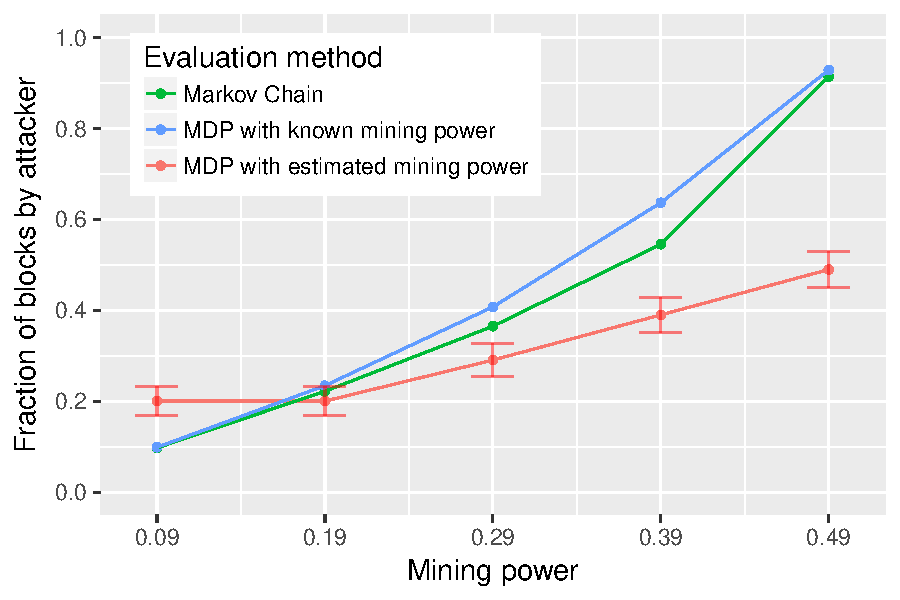
\includegraphics[width=0.9\textwidth]{graphs/problem}
	\caption{The green and blue lines show the results of the Markov chain of Eyal~\cite{eyal:2014} and the MDP of Gervais~\cite{Gervais:2016}, respectively. The red line shows the fraction of blocks owned by the attacker on the main chain, given his mining power.  Error bounds show 95\% confidence intervals; and the plot is the mean of 600 trials at that point, using estimated mining powers on the MDP of Gervais~\cite{Gervais:2016}. 
	\label{fig:RL}}
\end{center}\end{figure}

%We could also estimate the network-wide hash rate if we used {\em all} blocks instead of those by a specific miner. In Section~\ref{sec:time based} we have shown that the unbiased MLE estimator for $\beta$ is equation~\ref{eq:beta-hat}. Let $r$ be the miner's hash rate in minutes (i.e., the number of hashes per time unit), and $X = X_1, \dots, X_{n}$, where $X \sim$ Exp$(\beta)$, where $\beta = 1/\lambda$. We can use our estimate, $\hat{\beta}$, of $\beta$ to calculate a given miner's hash rate.
%%Note that $\lambda r$ is the expected number of hashes each time a block is created 
%\begin{align}
%\EX[h] = r \lambda &= r \frac{1}{\beta}  \\
%r &= \EX[h] \hat{\beta}
%\end{align}
%A miner's estimated hash rate 
%given target $T_i$ and $n$ inter-arrival times for $n+1$ blocks discovered by that miner is 
%\begin{align}
%\frac{(2^{256}-1)\hat{\beta}_m}{T_i}.
%\end{align}
%The entire network's estimated hash rate 
%given target $T_i$ and $n$ inter-arrival times for $n+1$ blocks is 
%\begin{align}
%\frac{(2^{256}-1)\hat{\beta}}{T_i}.
%\end{align}
%The miner's mining power, $\psi$, is the entire network's hash rate over his hash rate:
%\begin{align}
%%\psi &= \frac{\sfrac{(2^{256}-1)\hat{\beta}}{T_i}}{\sfrac{(2^{256}-1)\hat{\beta}_m}{T_i}} \\
%&= \frac{\hat{\beta}}{\hat{\beta}_m}
%\end{align} 
%\para{Expected Value of Hash Rate.}
%\begin{align}
%\EX[r|T_i,X_1,...,X_n] &= \EX\bigg[\frac{(2^{256}-1)\hat{\beta}}{T_i}\bigg] \\
%&= \frac{(2^{256}-1)}{T_i}\EX[\hat{\beta}] \\
%&= \frac{(2^{256}-1)\beta}{T_i}
%\end{align}
%
%\para{Variance of Hash Rate.}
%The variance associated with this estimate is
%\begin{align}
%\text{Var}(\psi|X_1,...,X_n, X_1^m,...,X_n^m) &= \text{Var}\bigg(\frac{\hat{\beta}}{\hat{\beta}_m}\bigg) \\
%&= \bigg(\frac{\hat{\beta}_m}{\hat{\beta}}\bigg)^2 \frac{n(n+n-1)}{(n-2)(n-1)^2} \\
%&= \frac{\hat{\beta}_m^2}{\hat{\beta}^2} \frac{n(2n-1)}{(n-2)(n-1)^2}.
%\end{align}
%\begin{align}
%\text{Var}(r|T_i,X_1,...,X_n) &= \text{Var}\bigg(\frac{(2^{256}-1)\hat{\beta}}{T_i}\bigg) \\
%&= \frac{(2^{256}-1)^2}{T_i^2} \text{Var}(\hat{\beta}) \\
%&= \frac{(2^{256}-1)^2\beta^2}{T_i^2n}.
%\end{align}
%Because $0<\hat{\beta}<1, 0<\hat{\beta}_m<1$ and $\hat{\beta}_m > \hat{\beta}$, it follows that $\sfrac{\hat{\beta}}{\hat{\beta}}_m < 1$. Therefore, $\sfrac{n(2n-1)}{(n-2)(n-1)^2}$ is the upper bound on the variance. Equation 4.10 can be obtained from Equation 4.9 since the ratio of two Gamma distributions follows a compound Gamma distribution. \url{https://stats.stackexchange.com/questions/207595/distribution-of-the-ratio-of-two-gamma-random-variables}

%\para{Bias of Hash Rate.}
%\begin{align}
%\text{bias}(r|T_i,X_1,...,X_n) &= \EX[r|T_i,X_1,...,X_n] - r \\
%&= \frac{(2^{256}-1)\beta}{T_i} - \frac{(2^{256}-1)\beta}{T_i} \\
%&= 0
%\end{align}

%\para{Example.}
%The current Bitcoin Core difficulty, $D_i$, is $1,590,896,927,258 \approx 2^{40}$. Therefore, the current target, $T_i$, is
%\begin{align}
%T_i &= \frac{2^{224}}{D_i} = \frac{2^{224}}{2^{40}} \\
%&\approx 2^{184}.
%\end{align}
%Then the variance associated with hash rate estimation approximately is
%\begin{align}
%\text{Var}(r|T_i,X_1,...,X_n) &= \frac{(2^{256}-1)^2\beta^2}{T_i^2n} \\
%&\approx  \frac{(2^{256})^2\beta^2}{T_i^2n} \\
%&\approx  \frac{(2^{256})^2\beta^2}{(2^{184})^2n} \\
%&\approx  \frac{2^{512}\beta^2}{2^{368}n} \\
%&\approx  2^{144}\frac{\beta^2}{n}.
%\end{align}
%The variance associated with estimating hash rate for $0 \leq \beta \leq 1$ and for any $n \in \mathbb{Z}^+ $ is large. We need more blocks than those that are on the Bitcoin Core blockchain to reduce variance. RL provides a solution to this problem because it assumes that an agents acts in an environment where there is uncertainty. Therefore, we use RL methods to search for the optimal strategies for an attacker, who wants to perform attacks on blockchain networks. Then we compare the optimal policy found by RL algorithms to those cited in previous work.

\section{Preliminary Work}
Sapirshtein~\cite{sapirshtein:2015} and Gervais~\cite{Gervais:2016} use an {\em average reward} MDP for computing the optimal strategies for selfish mining and double spending. Average reward MDPs, as the name suggests, maximize an agent's average return instead of {\em episodic} MDPs that maximize absolute return over time. In the following section, we formulate the problem as an episodic MDP that is more widely studied and easier to solve.

\subsection{Formulating the Problem as an Episodic MDP}
\para{States.} Using the model model of Sapirshtein et al.~\cite{sapirshtein:2015} for selfish mining as a basis, we construct the following MDP that is a 6-tuple $\{S, A, P, R, \gamma, d_0\}$, where $S = \{(w, x, y, z, i, k)\}$ such that $w, x, y, z, i, k \in \mathbb{N}$. The state consists of a 6-tuple where each element represents the following: 1) $w$ is the number of blocks created by the honest miners on the main chain. 2) $x$ is the number of blocks created by the attacker. 3) $y$ is the number of attacker blocks that the honest network accepts as part of the main chain. 4) $z$ is a variable that represents the state of the main chain. If $z = 1$, the attacker performed a {\tt match} action, resulting in a fork on the main chain. If $z = 0$, the attacker mined the last block, and if $z = 2$, the honest network mined the last block, enabling the attacker to release a competing block if he has any. 5) $i$ is the number of attacker blocks on the main chain so far. 6) $k$ is the {\em total} number of blocks on the main chain so far. Note that this representation assumes that all blocks build on the same parent block.

\para{Actions.} $A = \{\texttt{adopt}, \texttt{mine}, \texttt{override}, \texttt{match}\}$. \texttt{adopt} refers to the adoption of the main chain, thereby discarding all blocks created by the attacker (except those already accepted on the main chain by the honest network). The action \texttt{mine} denotes that the attacker continues to mine, waiting to see who the next block will be discovered by. \texttt{override} refers to an attacker's releasing one more block than the honest miners' blocks on the main chain. This action can be viewed as honest or selfish depending on the current state. If the honest miners have no blocks on the main chain, an addition of a block to the main chain means that the attacker is honest. However, if the honest miners already have blocks on the main chain and the attacker releases an alternative chain that is 1 block longer than that created by the honest miners, then the attacker overwrites the main chain, wasting the victim's computational resources. The \texttt{match} action means that the attacker releases as many blocks as there are on the main chain, causing a bifurcation.

\para{Initial state distribution.} $d_0 = \{(0, 0, 0, 0, 0, 0)\}$, where $P(S_0 = (0, 0, 0, 0, 0, 0)) = 1$. In other words, the start state assumes that no blocks have been mined yet. If the attacker chooses to \texttt{adopt} and the length of the main chain is greater than some CUTOFF, the agent goes back to the start state.

\para{Transition Function.} We consider 3 of parameters of interest also included in the model of Gervais et al.~\cite{Gervais:2016}: $q$, CUTOFF and $a$. At each time step, a new block is created by the network: with probability $q$, where $q$ is the mining power of the attacker, the attacker is the winner of a new block. The honest network discovers a block with probability $1-q$. Not all actions are available in every state. The attacker can always choose to \texttt{mine} or \texttt{adopt}. If the attacker chooses an {\tt adopt} action, he discards all blocks he has created on his alternative chain and accepts the blocks on the main chain created by the honest network should there exist any. Furthermore, \texttt{override} and \texttt{match} are only available when the attacker has enough blocks and the last block has been mined by the honest network. At CUTOFF $= 75$, the length of the main chain is equal to or longer than 75 blocks, and we force the attacker to \texttt{adopt} in order to have episodic trials. Our third parameter, $a$, represents network connectivity. If there is a fork of same length on the main chain, fraction $a$ of the honest miners build on the attacker's alternative chain. We set $a=1$ to give advantage to the attacker, and to analyze if RL methods can learn to take advantage of the \texttt{match} action. Therefore, in our formulation, if the attacker matches the main chain with a fork of the same length, all honest miners build on the attacker's chain. 

\section{Proposed Work}\label{section:selfishRL-proposed-work}
We propose to complete the following tasks to extend this chapter:
\begin{enumerate}
\item Prove that the episodic MDP presented above is equivalent to the average reward MDP of Sapirshtein et al.~\cite{sapirshtein:2015}.
\item Evaluate the model of Sapirshtein et al.~\cite{sapirshtein:2015} where an agent first calculates the hash rate of the attacker using our estimator.
\item Run RL algorithms such as Q-learning and SARSA on the MDP presented, where network parameters are not revealed to an agent.
\item Compare the performance of RL algorithms to previous work.
\item Evaluate RL algorithms on the model of Sapirshtein et al.~\cite{sapirshtein:2015} when the mining power of the network is fluctuating.
\end{enumerate}

